
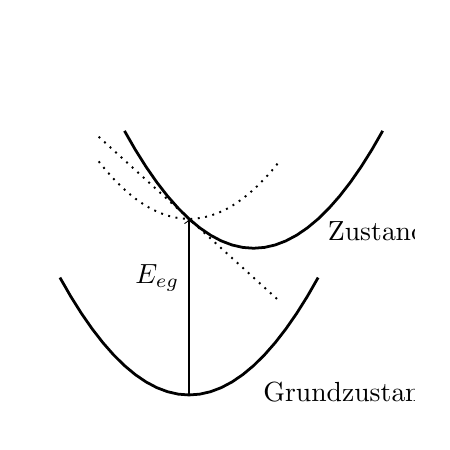
\begin{tikzpicture}
\useasboundingbox (0,0) rectangle (5,5);

\begin{axis}[no markers, 
        domain=-1:1.5,
         axis y line=none,
           axis x line=none,
           width= 6.5cm]
\addplot [domain=-1:1,  line width=1pt]    {x^2};
\addplot  [domain=-0.5:1.5, line width=1pt]    {x^2 + 1.5 - x};

\addplot  [dotted, domain=-0.7:0.7, line width=0.7pt] {1.5 - x};
\addplot  [dotted, domain=-0.7:0.7, line width=0.7pt] {1.5 + x^2};

\addplot[->] coordinates
           {(0,0) (0, 1.5)};

\node[anchor=east] at (axis cs: 0,1) {$E_{eg}$};
\node[anchor= west] at (axis cs: 0.5,0) {Grundzustand $g$};
\node[anchor=west] at (axis cs: 1,1.4) {Zustand $e$};
           
\end{axis}

\end{tikzpicture}
